\documentclass[11pt,a4paper,twoside]{article}
\usepackage[utf8]{inputenc}
\usepackage[T1]{fontenc}

\usepackage{mathptmx}
\usepackage{datetime}
\usepackage[spanish, es-nolists]{babel}
\usepackage{amsmath}
\usepackage{amsthm}
\usepackage{amsfonts}
\usepackage{amssymb}
\usepackage{titlesec}
\usepackage{graphicx}
\usepackage{mathtools}

\decimalpoint

\usepackage{array}
\usepackage{float}
\usepackage[a4paper]{geometry}
\geometry{top=2.5cm, bottom=2cm, left=2.54cm, right=2.54cm}
\usepackage{fancyhdr}
\pagestyle{fancy}
\fancyhf{}  % Limpiar los encabezados y pies de página predeterminados
% Encabezados para páginas impares
\fancyhead[LE,RO]{\thepage} % En la izquierda de la página impar
\fancyhead[RE]{\textsc{Garbayo, I.}} % En la derecha de la página impar
% Encabezados para páginas pares
\fancyhead[LO]{\textit{Generación y optimización de código}}  % En la izquierda de la página par
\fancyfoot{}

\usepackage{color}
\usepackage{cancel}
\usepackage{ulem}
\usepackage{tcolorbox}
\usepackage{multirow}
\usepackage{tikz}
\usetikzlibrary{babel, arrows.meta, arrows, datavisualization, patterns}
\usepackage{multicol}
\usepackage{stackrel}
\usepackage{pdfpages}
\renewcommand{\labelitemi}{\textbullet}

\theoremstyle{definition}
\newtheorem{ejemplo}{\textbf{Exemplo}}
\newtheorem{ejer}{\textcolor{red}{\textbf{Exercicio}}}
\newtheorem{defi}{\textbf{Definición}}
\newtheorem{theorem}{\textbf{Teorema}}
\newtheorem{lema}{\textbf{Lema}}
\newtheorem{corol}{\textbf{Corolario}}
\newtheorem{prop}{\textbf{Proposición}}
\newtheorem{nota}{\textbf{\textit{Nota}}}

\renewcommand\qedsymbol{$\blacksquare$}

\usepackage{hyperref}
\hypersetup{
	colorlinks,
	citecolor=black,
	filecolor=black,
	linkcolor=black,
	urlcolor=black
}

\usepackage{enumitem}


\newcommand{\imagen}[1]{
	\begin{figure} [H] \centering
		\includegraphics[width=\textwidth]{#1}
	\end{figure}
}

\title{%
	\LARGE \textbf{Compiladores e Intérpretes} \\ \vspace*{1cm} \textbf{Práctica 1: Generación y optimización de código}
	\\ \Large \textbf{Suavizado de una imagen en gris mediante vecindades $5\times 5$}}
\author{\textsc{Ignacio Garbayo Fernández}}
\date{Universidade de Santiago de Compostela}

\setlength{\parskip}{5pt}

\usepackage{setspace}

%\onehalfspacing % Configura el interlineado a 1.5

\setlength{\parindent}{0.7cm}

\usepackage[hang, small,labelfont=bf,up,textfont=up]{caption}
\usepackage{hanging}
\usepackage{sectsty}

\sectionfont{\fontsize{14}{15}\selectfont}
\subsectionfont{\fontsize{12}{15}\selectfont}
\subsubsectionfont{\fontsize{12}{15}\selectfont}

\usepackage{titlesec}
\titleformat{\subsection}[block]{\normalfont\large\itshape}{\thesubsection}{1em}{}
\titlespacing*{\section}
{0pt}{\baselineskip}{0pt}
\titlespacing*{\subsection}
{0pt}{\baselineskip}{0pt}
\titlespacing*{\subsubsection}
{0pt}{\baselineskip}{0pt}

\usepackage[cache=false]{minted}
\definecolor{bg}{rgb}{.95, .95, .95}

\usepackage[backend=biber, style=ieee, sorting=nty]{biblatex}
\bibliography{references}


\begin{document}
	
	% PORTADA
	\maketitle
	\thispagestyle{empty}
	
	\vspace*{1cm}
	
	% ÍNDICE
	\renewcommand{\contentsname}{Índice} % Cambia el título
	\tableofcontents


	\newpage


	\section{Introducción}
	
	El objetivo de esta práctica es analizar el impacto del orden de anidamiento de los bucles en el rendimiento temporal de una operación de suavizado aplicada a imágenes en escala de grises. Dicha operación se implementa en lenguaje C utilizando una vecindad cuadrada de tamaño $5\times 5$. Se evalúan las 24 permutaciones posibles de los 4 índices principales, buscando identificar cuál proporciona el mejor rendimiento en términos de tiempo de ejecución. Además, se estudia el efecto de diferentes opciones de compilación: la optimización básica \texttt{-O1} y la versión con desenrollado de bucles (\texttt{-O1 -funroll-loops}). Para ello, se comparan los códigos ensamblador generados por ambas opciones y se analizan los tiempos de ejecución resultantes sobre imágenes de distintos tamaños, con el fin de entender mejor cómo influyen estas decisiones de implementación y compilación en la eficiencia del programa.
	
	La comparación entre los diferentes códigos ensamblador permitirá ver cómo afectan las transformaciones del compilador al resultado final, facilitando una comprensión más profunda de la optimización a bajo nivel. Además, se podrá determinar qué orden de anidamiento de los índices minimiza el tiempo de ejecución, lo cual está directamente relacionado con la localidad de memoria y la jerarquía de caché del procesador.
	

	\section{Descripción de la técnica}
	
	Para la práctica, se propone estudiar el rendimiento de varias técnicas que implementen la expresión (\ref{eq}).
	
	\begin{equation} \label{eq}
		I^\prime (i,j) = \dfrac{1}{25}\, \sum_{m=-2}^2 \sum_{n=-2}^2 I(i+m, j+n).
	\end{equation}

	El orden inicial y natural de los bucles, que denotaremos por \texttt{ijmn}, se muestra en la siguiente porción de código.
	
	\begin{minted}[linenos, fontsize=\small, bgcolor=bg]{c}
for (int i = 0; i < N; ++i) {
	for (int j = 0; j < M; ++j) {
		float sum = 0.0;
		int count = 0;
		for (int m = -2; m <= 2; ++m) {
			for (int n = -2; n <= 2; ++n) {
				int x = i + m;
				int y = j + n;
				if (x >= 0 && x < N && y >= 0 && y < M) {
					sum += I[x][y];
					count++;
				}
			}
		}
		Iprime[i][j] = sum / count;
	}	
}
	\end{minted}

	Para las ejecuciones, se probará con todas las permutaciones posibles de los índices anteriores, resultando en 24 ordenaciones diferentes de los bucles para efectuar la misma operación.
	
	Conviene resaltar que, para poder evaluar todas las permutaciones posibles del orden de los bucles de manera coherente y comparable, el algoritmo de suavizado se ha implementado en dos fases claramente diferenciadas. En la fase 1 (\textbf{acumulación}), los bucles se reordenan libremente según cada una de las 24 combinaciones posibles, y en esta etapa se acumulan las contribuciones de los píxeles vecinos en matrices auxiliares \texttt{sum[][]} y \texttt{count[][]}, que almacenan respectivamente la suma de los valores y el número de contribuciones por píxel. En la fase 2 (\textbf{normalización}), los bucles se mantienen fijos recorriendo las coordenadas \texttt{i} y \texttt{j} de la imagen para calcular el valor promedio de cada píxel dividiendo la suma acumulada por el contador correspondiente. Además, para facilitar el análisis posterior, se ha implementado una gestión automática de directorios, organizando los resultados obtenidos según la permutación de bucles utilizada y el tamaño de la imagen procesada, lo que permite un acceso ordenado y sistemático a los datos experimentales.
	
	La fase de acumulación presenta el esquema siguiente. a estructura de este bloque se genera automáticamente para cada una de las 24 permutaciones posibles de esos cuatro índices. Cada permutación produce un bloque de bucles anidados con este patrón general.
	\begin{minted}[linenos, fontsize=\small, bgcolor=bg]{c}
for (var1) {
	for (var2) {
		for (var3) {
			for (var4) {
				// Cálculo del píxel vecino
				int x = i + m;
				int y = j + n;
				if (x >= 0 && x < N && y >= 0 && y < M) {
					sum[i][j] += I[x][y];
					count[i][j]++;
				}
			}
		}
	}
}
	\end{minted}
	
	Por su parte, la fase de normalización tiene siempre el mismo código C.
	\begin{minted}[linenos, fontsize=\small, bgcolor=bg]{c}
// Fase de normalización
for (i = 0; i < N; ++i) {
		for (j = 0; j < M; ++j) {
				Iprime[i][j] = (count[i][j] != 0) ?
				sum[i][j]/count[i][j] : 0.0f;
		}
}
	\end{minted}

	Este enfoque modular permite comparar el impacto del orden de recorrido sobre el rendimiento del algoritmo y facilita la experimentación sistemática con distintas configuraciones.
	
	
	\subsection{Configuración del experimento}
	
	El objetivo del experimento es múltiple. En primer lugar, se identificará la permutación más eficiente de los bucles. Se podrá determinar qué \textbf{orden de anidamiento} de los bucles minimiza el tiempo de ejecución, lo cual está directamente relacionado con la localidad de memoria y la jerarquía de caché del procesador. Cada orden se denotará de la forma (\ref{indices}).
	
	\begin{equation} \label{indices}
		\{\text{índice 1}\}\{\text{índice 2}\}\{\text{índice 3}\}\{\text{índice 4}\}.
	\end{equation}

	Algunos ejemplos son \texttt{ijmn}, \texttt{jinm} o \texttt{njim}.
	
	Además, se comparará el impacto de las \textbf{opciones de compilación}. Al analizar los tiempos y los códigos ensamblador con \texttt{-O1} y \texttt{-O1} \texttt{-funroll-loops}, se podrá ver si el desenrollado de bucles mejora o empeora el rendimiento, y en qué casos.
	
	Otro interés de la práctica es evaluar la escalabilidad del rendimiento. Al usar imágenes de \textbf{distintos tamaños} ($\texttt{N} \times \texttt{M}$), se podrá estudiar cómo varía el tiempo de ejecución en función del tamaño de los datos, lo que ayuda a entender la eficiencia del algoritmo a mayor escala. Para este particular, utilizamos matrices almacenadas de forma estática, para no sacrificar rendimiento en el acceso, y por lo tanto probamos con tamaños de problema no demasiado grandes. Estos se pueden ver en \ref{eq:n} y \ref{eq:m}.
	
	\begin{equation} \label{eq:n}
		N = \left( \begin{matrix}
			120, & 250, & 380, & 510, & 600
		\end{matrix} \right),
	\end{equation}

	\begin{equation} \label{eq:m}
		M = \left( \begin{matrix}
			120, & 250, & 380, & 510, & 600
		\end{matrix} \right).
	\end{equation}
	
	Al ya efectuarse el experimento mediante un doble bucle sobre cada uno de los valores de \texttt{N} y \texttt{M} mostrados en (\ref{eq:n} y \ref{eq:m}), no es necesario definir un número \texttt{ITER} para evitar el ruido, como sí se hace en la Práctica 2 de la asignatura.

	Para cada combinación de \texttt{N}, \texttt{M}, orden de bucles y optimización (4 variables), es fundamental ejecutar el algoritmo un número suficiente de veces, denotado por \texttt{REPS}, con el fin de obtener medidas de rendimiento representativas y estables. La variabilidad inherente al sistema ---debido a factores como la planificación del sistema operativo, el estado de la caché, o procesos en segundo plano--- puede provocar fluctuaciones significativas en los tiempos de ejecución individuales. Al repetir las mediciones y calcular posteriormente estadísticas como la \textbf{media}, se obtiene una caracterización más completa del comportamiento del algoritmo. Estas métricas permiten representar en las gráficas no solo la tendencia central, sino también la dispersión y los extremos del rendimiento, ofreciendo una visión más realista y robusta para comparar implementaciones o analizar cuellos de botella. Para este particular, \texttt{REPS} se fija a 100, un número suficientemente grande, como se comentó en clase.
	
	
	\subsection{Interpretación gráfica}
		
	El suavizado de una imagen en escala de grises puede interpretarse visualmente como un proceso en el que se reemplaza cada píxel por el promedio de los valores de intensidad de una vecindad centrada en él. 
	
	La imagen se puede representar como una cuadrícula bidimensional, donde cada celda contiene un valor de intensidad entre 0 y 255. Para cada píxel $(i,j)$, se toma una submatriz centrada en ese punto que abarca los píxeles desde $(i-2, j-2)$ hasta $(i+2, j+2)$. Esta región incluye 25 píxeles (el propio y sus vecinos inmediatos). Se puede ver en \ref{matriz}.
	
	\begin{equation} \label{matriz}
		\begin{bmatrix}
			x & x & x & x & x \\
			x & x & x & x & x \\
			x & x & \boxed{O} & x & x \\
			x & x & x & x & x \\
			x & x & x & x & x
		\end{bmatrix},
	\end{equation}
	
	donde $O$ indica el píxel central $(i,j)$. 
	
	El nuevo valor $I^\prime(i,j)$ se obtiene calculando la media de los 25 valores dentro de la vecindad. Este proceso tiene varios efectos visuales importantes, como las siguientes.
	
	\begin{itemize}
		\item \textbf{Reducción de ruido.} Las variaciones locales se atenúan al ser promediadas.
		\item \textbf{Desenfoque.} Los bordes y detalles finos pierden nitidez.
		\item \textbf{Suavizado visual.} La imagen resultante presenta transiciones más suaves entre regiones de diferente intensidad.
	\end{itemize}
	
	En conjunto, este tipo de suavizado actúa como un filtro de promedio que mejora la homogeneidad de la imagen a costa de perder cierta cantidad de detalle. La Figura \ref{transi} muestra un ejemplo de aplicación de estas técnicas.
	
	\begin{figure} [H] \centering
		\includegraphics[width=.45\textwidth]{imagenes/entrada.pdf}
		\hspace*{0.5cm}
		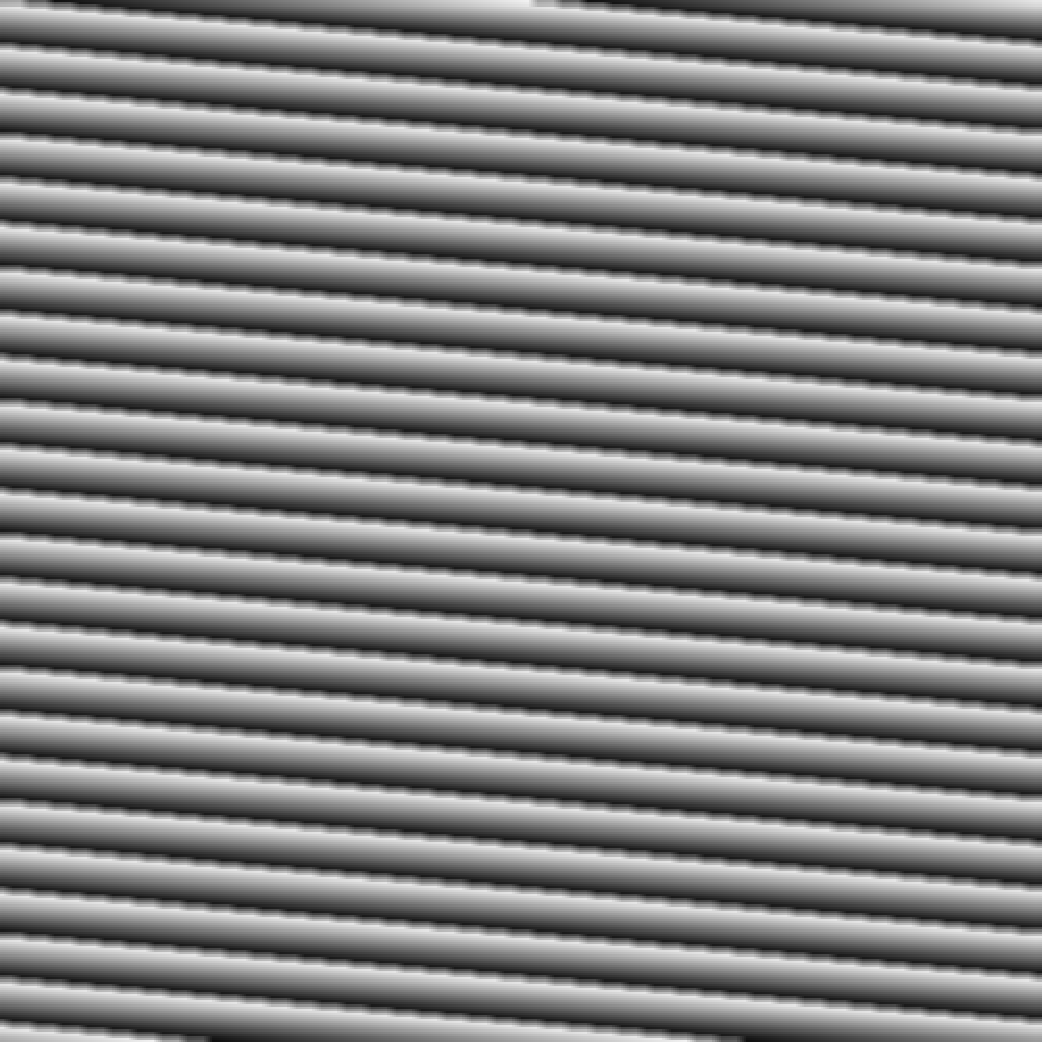
\includegraphics[width=.45\textwidth]{imagenes/salida.pdf}
		\caption{Ejemplo de antes y después de una imagen al aplicarle el suavizado que se describe durante la práctica.}
		\label{transi}
	\end{figure}
	
	Las imágenes de la Figura \ref{transi} se han generado utilizando la función de C que aparece a continuación.
	\begin{minted}[linenos, fontsize=\small, bgcolor=bg]{c}
#include <string.h>
void guardar_imagen(char* nombre_imagen, float I[N][M]) {
	// Guardar la imagen
	FILE *f = fopen(nombre_imagen, "w");
	fprintf(f, "P2\n%d %d\n255\n", M, N);
	for (int i = 0; i < N; ++i) {
		for (int j = 0; j < M; ++j) {
			int val = (int)(I[i][j]);
			if (val < 0) val = 0;
			if (val > 255) val = 255;
			fprintf(f, "%d ", val);
		}
		fprintf(f, "\n");
	}
	fclose(f);
}
	\end{minted}
	
	
	\section{Beneficios y desventajas esperados de las técnicas de optimización}

	El compilador GCC proporciona distintos niveles de optimización que pueden activarse mediante diferentes opciones.
	
	De acuerdo a \cite{gcc}, el nivel \texttt{-O1} introduce un conjunto básico de optimizaciones que buscan reducir tanto el tamaño como el tiempo de ejecución del código sin aumentar demasiado el tiempo de compilación. Entre las optimizaciones activadas en este nivel se incluyen:
	
	\begin{itemize}
		\item Eliminación de código muerto, es decir, instrucciones que nunca se ejecutan o cuyos resultados no se utilizan.
		\item Propagación de constantes, que sustituye expresiones por sus valores constantes cuando sea posible.
		\item Eliminación de operaciones redundantes, como comparaciones duplicadas o asignaciones innecesarias.
		\item Fusión de ajustes de pila consecutivos para mejorar la eficiencia en llamadas a funciones.
		\item Omisión del puntero de marco en funciones simples, lo que reduce el uso de registros.
	\end{itemize}
	
	Este nivel es especialmente adecuado para programas grandes generados automáticamente, donde se desea un equilibrio entre rendimiento y consumo de memoria durante la compilación.
	
	Por su parte, la opción \texttt{-funroll-loops} del nivel \texttt{O1} desenrolla bucles cuando el compilador puede determinar el número de iteraciones en tiempo de compilación. El desenrollado consiste en replicar el cuerpo del bucle varias veces dentro del propio bucle para reducir la sobrecarga del control de iteración (como incrementar índices o comparar condiciones).
	
	Según \cite{aho}, en la programación basada en regiones, el límite de una iteración de un ciclo actúa como una barrera para el movimiento de código, impidiendo que las operaciones de una iteración se traslapen con las de otra. Una técnica simple pero muy efectiva para mitigar este problema es el \textit{desenrollamiento de bucles} (\textit{loop unrolling}), que consiste en replicar el cuerpo del ciclo un pequeño número de veces antes de aplicar técnicas de planificación global del código.
	
	Este proceso introduce múltiples instancias de las instrucciones dentro del cuerpo del bucle, lo cual amplía las oportunidades para que los algoritmos de planificación global identifiquen y exploten paralelismo entre operaciones.
	
	El desenrollamiento de ciclos mejora el rendimiento al permitir el traslape de cálculos entre iteraciones sucesivas. Sin embargo, el límite del ciclo desenrollado sigue funcionando como una barrera para el movimiento de código. Por tanto, aunque esta técnica proporciona mejoras notables, todavía deja un margen de rendimiento potencial sin explotar.
	
	Esto, en la práctica considerada, permite reducir el número de saltos e instrucciones de control, pudiendo aumentar el paralelismo del \textit{pipeline} de instrucciones. A menudo mejora el rendimiento si el acceso a memoria tiene buena localidad, pero solo se aplica cuando el número de iteraciones es conocido o puede inferirse. Además, puede aumentar el tamaño del código significativamente, lo que en algunos casos perjudica la caché de instrucciones.
	
	\section{Programación y código en ensamblador}
	
	\subsection{Arquitectura de compilación y ejecución}
	
	La compilación con la opción \texttt{-S} de GCC produce códigos fuente del ensamblador de la máquina mediante los que podemos analizar la traducción de las 2 estrategias. Se han ejecutado los códigos en una máquina ASUS Zenbook UX425EA 1.0, equipada con el sistema operativo Ubuntu 22.04.3 LTS x86\_64. Cuenta con un procesador Intel i7-1165G7 de 4 núcleos físicos de undécima generación, que funciona a una frecuencia de reloj de 2.80 GHz. Las direcciones de memoria ocupan 39 bits físicos y 48 bits virtuales.
	
	Cada núcleo dispone de 2 hilos de procesamiento, resultando en un total de 8 hilos. Dispone de 16 GiB de memoria RAM totales y de 4 niveles de memoria caché: L1d (192 KiB, 4 instancias), L1i (128 KiB, 4 instancias), L2 (5 MiB, 4 instancias) y L3 (12 MiB, 1 instancia). El TDP (\textit{Thermal Design Power}) es configurable entre 12 y 28 W. Se omite la inclusión de otros componentes como la tarjeta gráfica o de sonido porque no afectarán a los resultados de las pruebas. La versión del compilador utilizada es GCC 11.4.0.

	Con el fin de ejecutar todas las 48 versiones (24 órdenes con 2 niveles de optimización) en las mismas condiciones, el envoltorio de declaraciones y variables de medición previos a las llamadas correspondientes ha sido el que se muestra a continuación.
	
	Conviene mencionar que las mediciones se han efectuado utilizando la función \texttt{clock\_gettime()}, pues aporta una precisión de nanosegundos, necesaria para poder comparar las versiones compiladas con las diferentes opciones.
	
	\begin{minted}[linenos, fontsize=\small, bgcolor=bg]{c}
float I[N][M], Iprime[N][M];
int i, j, m, n;

// Abrir fichero de escritura
if (argc < 2) { ... }
nombre_archivo = argv[1];
FILE* file = fopen(nombre_archivo, "a");
if (file == NULL) { ... }

// Calentamiento de la caché
for (int i = 0; i < N; ++i) {
	for (int j = 0; j < M; ++j) {
		// Inicializamos I con patrón simple tipo tablero
		I[i][j] = (float)((i * M + j) % 256);
		Iprime[i][j] = 0.0f;
	}
}

// Medir el overhead e inicio
clock_gettime(CLOCK_MONOTONIC, &overhead);
clock_gettime(CLOCK_MONOTONIC, &inicio);

// algoritmo

// Medir el final
clock_gettime(CLOCK_MONOTONIC, &final);
// Cálculo de tiempos
tiempo_overhead = (inicio.tv_sec - overhead.tv_sec) + 
(inicio.tv_nsec - overhead.tv_nsec) / 1e9;
tiempo = (final.tv_sec - inicio.tv_sec) + (final.tv_nsec - inicio.tv_nsec) / 1e9;
tiempo = tiempo - tiempo_overhead;

// Imprimir en el archivo
fprintf(file, "%d\t%d\t%.9f\n", N, M, tiempo);

// Cerrar el archivo
fclose(file);
return 0;
	\end{minted}

	\subsection{Ordenamiento de bucles}
	
	Podemos intentar comparar el código en ensamblador entre órdenes distintos, por ejemplo, \texttt{ijmn} y \texttt{jnmi}, ambas en sus versiones \texttt{-O1}, para fijar una opción de complación concreta.
	
	Ambas versiones del programa han sido compiladas con la opción de optimización \texttt{-O1}, pero el orden de anidamiento de los bucles (\texttt{ijmn} frente a \texttt{jnmi}) produce diferencias claras en el ensamblado generado. A pesar de que el número total de iteraciones es el mismo, el patrón de bucles influye directamente en la estructura del código a bajo nivel.
	
	En la versión \texttt{ijmn}, los bucles aparecen estructurados de forma más lineal, con bloques repetidos para simular anidamientos mediante etiquetas como \texttt{.L4}, \texttt{.L5}, \texttt{.L20}, etc. En cambio, la versión \texttt{jnmi} presenta una jerarquía de bucles más profunda, con etiquetas que se entrelazan y reaprovechan en distintos niveles (\texttt{.L13}, \texttt{.L11}, \texttt{.L8}, etc.). Esto refleja una diferencia en cómo el compilador interpreta el control de flujo según el orden de los bucles.
		
	Por otra parte, en \texttt{ijmn}, los contadores de bucle suelen almacenarse en los registros \texttt{\%eax} y \texttt{\%edx}. En la versión \texttt{jnmi}, debido a la mayor cantidad de bucles internos activos simultáneamente, el compilador utiliza además \texttt{\%ecx} y \texttt{\%esi}, indicando una necesidad de gestionar más niveles de control de bucle.
		
	Finalmente, la estructura de \texttt{jnmi} genera una mayor cantidad de saltos condicionales y anidados, lo cual puede dificultar la predicción de saltos por parte del procesador. En cambio, \texttt{ijmn} mantiene un flujo de ejecución más plano y repetitivo, aunque potencialmente menos eficiente si los accesos a memoria no están alineados con la organización natural de los datos.
	
	En resumen, el orden de los bucles (no solo de estos dos, sino para cualquiera de las 24 permutaciones) afecta no solo a la semántica del programa, sino también a su representación a bajo nivel. Esto puede tener implicaciones relevantes en el rendimiento debido a diferencias en la estructura de control, uso de registros, y la interacción con la jerarquía de memoria del sistema.
	
	
	\subsection{Opciones de compilación}
	
	Vamos a centrarnos en la traducción de los bucles de \texttt{algoritmo}, fijando para ello la ordenación inicial, \texttt{ijmn}. 
	
	La diferencia más significativa entre las versiones de ensamblador generadas por GCC con las opciones \texttt{-O1} y \texttt{-O1 -funroll-loops} se encuentra en el tratamiento de los bucles utilizados para simular carga computacional. Estos bucles, que consisten en contar regresivamente desde 600, son optimizados de manera diferente según la opción de compilación utilizada.
	
	En la versión solo con \texttt{-O1}, el bucle se compila como un ciclo simple que decrementa el registro en una unidad en cada iteración, como sigue.
	\begin{minted}[linenos, fontsize=\small, bgcolor=bg]{nasm}
movl    $600, %eax
.L5:
subl    $1, %eax
jne     .L5
	\end{minted}
	
	Este código realiza 600 iteraciones, con una operación de resta y una comparación por iteración.
	
	Cuando se activa la opción \texttt{-funroll-loops}, el compilador desenrolla el bucle, reduciendo la frecuencia de las operaciones de control de flujo:
	
	\begin{minted}[linenos, fontsize=\small, bgcolor=bg]{nasm}
movl    $600, %ecx
.L5:
subl    $8, %ecx
jne     .L5
	\end{minted}
	
	En este caso, se realiza una resta de 8 por iteración, reduciendo el número de ciclos de 600 a aproximadamente 75. Esto disminuye el número de saltos condicionales, lo cual puede mejorar el rendimiento si el bucle es crítico.
	
	Además, la versión con \texttt{-funroll-loops} emplea un conjunto más amplio de registros (\texttt{\%r8d}, \texttt{\%r9d}, \texttt{\%r10}, \texttt{\%r11}, \texttt{rcx}, etc.), en comparación con la versión básica que usa principalmente \texttt{\%eax} y \texttt{\%edx}. Este uso más sofisticado de registros permite reducir dependencias entre instrucciones y facilita una ejecución más eficiente.
	
	En resumen, la opción \texttt{-funroll-loops} introduce mejoras en eficiencia mediante el desenrollado de bucles simples, reduciendo el número de instrucciones de control de flujo y explotando mejor los recursos del procesador. Este tipo de optimización puede tener un impacto positivo en el rendimiento cuando los bucles implicados son lo suficientemente largos o frecuentes.
											
	
	\section{Resultados obtenidos}
	
	Los experimentos se han realizado teniendo en cuenta los parámetros \texttt{N}, \texttt{M} y \texttt{REPS} explicados en la sección 2. Las fases del experimento también se han introducido en la sección 4. En primer lugar, se realiza el calentamiento de la caché. Las matrices \texttt{I} y \texttt{Iprime} se llenan de valores flotantes entre 0 y 255 para que ya puedan estar disponibles en niveles altos de la caché. 
	
	A continuación, se obtiene el \textit{overhead}, medición que tiene como objetivo estimar el tiempo que tarda en ejecutarse la propia medición del tiempo. Esto se aproxima calculando el tiempo que se tarda en usar \texttt{clock\_gettime()} dos veces seguidas.
	
	A continuación, se describen las fases del análisis experimental desarrolladas para obtener conclusiones ordenadas.
	
	\subsection{Orden de anidamiento más eficiente}
	
	Una aproximación inicial, fijando dos valores $\texttt{N}=510$ y $\texttt{M}=510$, nos puede dar una idea intuitiva y poco precisa sobre cual puede ser el orden de anidamiento de bucles más eficiente.
	
	Para contar con esta intuición ejecutamos el experimento en las 48 versiones de las que disponemos. La Figura \ref{graf1} muestra tiempos de ejecución en segundos para todas estas ejecuciones, representando la media para cada combinación orden de índices y optimización.
	
	\begin{figure} [H] \centering
		\includegraphics[width=\textwidth]{../graficas/tiempos_N510_M510.pdf}
		\caption{Tiempos de ejecuión en segundos para un tamaño de problema fijado.}
		\label{graf1}
	\end{figure}

	A partir de la Figura \ref{graf1}, es esperable que las versiones que utilicen los órdenes \texttt{ijmn} o \texttt{ijnm} se ejecuten de forma más eficiente.
	
	Debemos hacer un análisis riguroso para asegurar esta afirmación. Para ello, repetimos el experimento anterior pero para todas las combinaciones de valores de \texttt{N} y \texttt{M} que se han contemplado en las expresiones (\ref{eq:n}) y (\ref{eq:m}). De aquí, podemos extraer los resultados del Cuadro \ref{graf2}.
	
	\begin{table}[H]
		\centering
		\begin{tabular}{|c|c|c|c|c|c|c|}
			\hline
			\textbf{\texttt{N}} & \textbf{\texttt{M}} & \textbf{Mejor \texttt{-O1}} & \textbf{Media \texttt{-O1}} & \textbf{Mejor \textit{unroll}} & \textbf{Media \textit{unroll}} & \textbf{\% Dif.} \\
			\hline
			120 & 128 & \texttt{ijmn} & 1.090326e-05 & \texttt{ijmn} & 2.4261e-06 & -77.75 \\
			120 & 256 & \texttt{ijmn} & 2.082725e-05 & \texttt{jinm} & 4.60312e-06 & -77.9 \\
			120 & 380 & \texttt{ijmn} & 2.881909e-05 & \texttt{ijmn} & 5.3074e-06 & -81.58 \\
			120 & 510 & \texttt{ijmn} & 3.767804e-05 & \texttt{ijnm} & 5.83417e-06 & -84.52 \\
			120 & 600 & \texttt{ijnm} & 4.344787e-05 & \texttt{ijnm} & 7.72611e-06 & -82.22 \\
			250 & 128 & \texttt{ijmn} & 2.401448e-05 & \texttt{ijnm} & 5.09881e-06 & -78.77 \\
			250 & 256 & \texttt{ijnm} & 4.295525e-05 & \texttt{ijnm} & 9.41980e-06 & -78.07 \\
			250 & 380 & \texttt{ijnm} & 5.554640e-05 & \texttt{ijmn} & 1.050918e-05 & -81.08 \\
			250 & 510 & \texttt{ijmn} & 7.662577e-05 & \texttt{ijmn} & 1.255755e-05 & -83.61 \\
			250 & 600 & \texttt{ijnm} & 8.549204e-05 & \texttt{ijmn} & 1.611574e-05 & -81.15 \\
			380 & 128 & \texttt{ijmn} & 3.474053e-05 & \texttt{ijmn} & 8.38551e-06 & -75.86 \\
			380 & 256 & \texttt{jimn} & 1.1251753e-04 & \texttt{ijmn} & 1.436288e-05 & -87.23 \\
			380 & 380 & \texttt{ijmn} & 9.034398e-05 & \texttt{ijmn} & 1.609858e-05 & -82.18 \\
			380 & 510 & \texttt{jinm} & 1.8641963e-04 & \texttt{ijnm} & 1.861935e-05 & -90.01 \\
			380 & 600 & \texttt{ijmn} & 2.1438295e-04 & \texttt{ijmn} & 2.38483e-05 & -88.88 \\
			510 & 128 & \texttt{ijmn} & 4.570822e-05 & \texttt{ijnm} & 1.070927e-05 & -76.57 \\
			510 & 256 & \texttt{ijmn} & 8.398133e-05 & \texttt{ijnm} & 1.994445e-05 & -76.25 \\
			510 & 380 & \texttt{ijmn} & 1.41235e-04 & \texttt{ijnm} & 2.236396e-05 & -84.17 \\
			510 & 510 & \texttt{ijnm} & 2.1954544e-04 & \texttt{ijmn} & 2.48581e-05 & -88.68 \\
			510 & 600 & \texttt{ijnm} & 2.8512295e-04 & \texttt{ijnm} & 3.503961e-05 & -87.71 \\
			600 & 128 & \texttt{ijmn} & 5.469117e-05 & \texttt{ijmn} & 1.293268e-05 & -76.35 \\
			600 & 256 & \texttt{ijnm} & 9.653618e-05 & \texttt{ijnm} & 2.399284e-05 & -75.15 \\
			600 & 380 & \texttt{ijmn} & 2.2010791e-04 & \texttt{ijnm} & 2.535058e-05 & -88.48 \\
			600 & 510 & \texttt{ijmn} & 2.6393468e-04 & \texttt{ijmn} & 3.045271e-05 & -88.46 \\
			600 & 600 & \texttt{ijmn} & 3.3417771e-04 & \texttt{ijnm} & 3.814898e-05 & -88.58 \\
			\hline
		\end{tabular}
		\caption{Comparación de versiones con y sin \textit{unroll} para distintas configuraciones $(\texttt{N}, \texttt{M})$.}
		\label{graf2}
	\end{table}
	
	Las frecuencias de aparición de los diferentes órdenes en el Cuadro \ref{graf2} son \texttt{ijmn} (29 veces), \texttt{ijnm} (19 veces), \texttt{jimn} (1 vez) y \texttt{jinm} (1 vez). Por lo tanto, concluimos que las secuencias de ordenado más eficientes, por una amplia mayoría experimental, son \texttt{ijmn} e \texttt{ijnm}.
	
	
	\subsection{Optimización sobre diferentes tamaños del problema}
	
	De acuerdo a los resultados del experimento desarrollado en la sección 5.1, vamos a fijar para este particular el orden \texttt{ijmn}, pues resultó ser el más rápido de todos. Con el fin de comparar las dos opciones de compilación introducidas en la sección 2, vamos a ejecutar el experimento sobre todas las combinaciones de \texttt{N} y \texttt{M} de las que disponemos para \texttt{-O1} y \texttt{-O1 -funroll-loops}.
	
	La Figura \ref{graf3} muestra un mapa de calor que representa el tiempo de ejecuión frente a los tamaños \texttt{N} y \texttt{M} para la optimización \texttt{-O1}.
	
	\begin{figure} [H] \centering
		\includegraphics[width=.8\textwidth]{../graficas/heatmap_ijmn_O1.pdf}
		\caption{Tiempos de ejecución para \texttt{-O1} con diferentes tamaños de problema.}
		\label{graf3}.
	\end{figure}

	Por otra parte, en la Figura \ref{graf4} muestra un mapa de calor con la misma información para la optimización \texttt{-O1 -funroll-loops}.
	
	\begin{figure} [H] \centering
		\includegraphics[width=.8\textwidth]{../graficas/heatmap_ijmn_O1_unroll.pdf}
		\caption{Tiempos de ejecución para \texttt{-O1} con \textit{unrolling} para diferentes tamaños de problema.}
		\label{graf4}.
	\end{figure}

	Al comparar las dos gráficas de calor (una para la versión sin \textit{unroll} y otra para la versión con \textit{unroll}), se pueden observar diferencias claras que justifican por qué la versión con \textit{unroll} es mejor en términos de rendimiento temporal. 

	La gráfica con \textit{unroll} muestra una distribución más regular y homogénea de los tiempos, con una clara tendencia a mantenerse en rangos bajos incluso a medida que aumentan los tamaños de \texttt{N} y \texttt{M}. Esto, junto con el Cuadro \ref{graf2}, muestra que la diferencia porcentual entre las dos opciones de compilación es sistemáticamente alta, con reducciones de entre un 75 \% y un 90 \% en el tiempo promedio respecto a la versión sin \textit{unroll}. Esto indica una mayor estabilidad del rendimiento frente al escalado del problema.
	
	
	\section{Conclusiones}
	
	A lo largo de todas las combinaciones evaluadas, la versión con bucles ordenados como \texttt{ijmn} ha producido sistemáticamente los mejores tiempos de ejecución, tanto con como sin optimización. Esta ordenación permite acceder a la imagen original $I(i+m, j+n)$ siguiendo un patrón de memoria contiguo que favorece la localidad espacial, reduciendo fallos de caché y mejorando la velocidad de acceso a datos.
	
	Por otra parte, el impacto del orden de bucles es tan relevante como las optimizaciones del compilador.  
	Aunque las opciones de compilación como \texttt{-funroll-loops} aportan mejoras notables, elegir un orden de bucles eficiente como \texttt{ijmn} proporciona una base sólida sobre la que dichas optimizaciones pueden actuar con mayor efectividad.
	
	En suma, la combinación de buen orden de bucles y optimizaciones resulta en el mejor rendimiento posible.  
	El mejor rendimiento se obtiene al combinar la ordenación \texttt{ijmn} con la opción \texttt{-O1 -funroll-loops}, lo que demuestra que el rendimiento depende tanto del diseño algorítmico como del uso adecuado de las capacidades del compilador.


\printbibliography
	
	

\end{document}